\documentclass[12pt,a4paper]{article}
\usepackage[utf8]{inputenc}
\usepackage{amssymb, amsmath, multicol}
\usepackage{mathtext}
\usepackage[russian]{babel}
\usepackage{graphicx}
\usepackage[shortcuts,cyremdash]{extdash}
\usepackage{wrapfig}
\usepackage{floatflt}
\usepackage{lipsum}
\usepackage{concmath}
\usepackage{euler}
\usepackage{tikz}  
\usepackage{longtable}
\usetikzlibrary{graphs}

\oddsidemargin=-15.4mm
\textwidth=190mm
\headheight=-32.4mm     
\textheight=277mm
\tolerance=100
\parindent=0pt
\parskip=8pt
\pagestyle{empty}
\renewcommand{\tg}{\mathop{\mathrm{tg}}\nolimits}
\renewcommand{\ctg}{\mathop{\mathrm{ctg}}\nolimits}
\renewcommand{\arctan}{\mathop{\mathrm{arctg}}\nolimits}
\newcommand{\divisible}{\mathop{\raisebox{-2pt}{\vdots}}}

\graphicspath{{pictures/}}

\author{Радькин Кирилл, Б01-005}
\title{Лабораторная работа 2.1.4. Определение теплоемкости твердых тел.}

\begin{document}
	\maketitle
	
	\paragraph* {Цель работы:} 1) измерение количества подведенного тепла и вызванного им нагрева твердого тела; 2) определение теплоемкости по экстраполяции отношения $\dfrac{\Delta Q}{\Delta T}$ к нулевым потерям тепла.
	
	\paragraph* {В работе используются:} калориметр с нагревателем и термометром сопротивления; амперметр; вольтметр; мост постоянного тока; источник питания 36 В.
	
	\paragraph* {Теоретическая справка:} В предлагаемой работе измерение теплоемкости твердых тел производится по обычной схеме. Исследуемое тело помещается в калориметр. Измеряется $\Delta Q$ — количество тепла, подведенного к телу, и $\Delta T$ — изменение температуры тела, произошедшее в результате подвода тепла. Теплоемкость определяется по формуле
	
	\begin{equation}
		C = \dfrac{\Delta Q}{\Delta T}
	\end{equation}
	
	Температура исследуемого тела надежно измеряется термометром (в нашем случае — термометром сопротивления), а определение количества тепла, поглощенного телом, обычно вызывает затруднение. В реальных условиях не вся энергия $P \Delta T$, выделенная нагревателем, идет на нагревание исследуемого тела и калориметра, часть ее уходит из калориметра благодаря теплопроводности его стенок. Оставшееся в калориметре количество тепла $\Delta Q$ равно
	
	\begin{equation}
		\Delta Q = P \Delta t - \lambda(T - T_k)\Delta t
	\end{equation}
	
	где $P$ — мощность нагревателя, $\lambda$ — коэффициент теплоотдачи стенок калориметра, $T$ — температура тела, $T_k$ — температура окружающего калориметр воздуха (комнатная), $\Delta t$ — время, в течение которого идет нагревание.\\
	Из уравнений (1) и (2) получаем
	
	\begin{equation}
		C = \dfrac{P - \lambda(T - T_k)}{\Delta T / \Delta t}
	\end{equation}
	
	Формула (3) является основной расчетной формулой работы. Она определяет теплоемкость тела вместе с калориметром. Теплоемкость калориметра должна быть измерена отдельно и вычтена из результата.\\
	С увеличением температуры исследуемого тела растет утечка энергии, связанная с теплопроводностью стенок калориметра. Из формулы (2) видно, что при постоянной мощности нагревателя по мере роста температуры количество тепла, передаваемое телу, уменьшается и, следовательно, понижается скорость изменения его температуры.\\
	Погрешности, связанные с утечкой тепла, оказываются небольшими, если не давать телу заметных перегревов и производить все измерения при температурах, мало отличающихся от комнатной $(T \rightarrow T_k)$. Однако при небольших перегревах возникает большая ошибка в измерении $\Delta T = T - T_k$ и точность определения теплоемкости не возрастает. Чтобы избежать этой трудности, в работе предлагается следующая методика измерений. Зависимость скорости нагревания тела $\Delta T / \Delta t$ от температуры измеряется в широком интервале изменения температур. По полученным данным строится график
	
	\begin{equation*}
		\dfrac{\Delta T}{\Delta t} = f(T)
	\end{equation*}
	
	Этот график экстраполируется к температуре $T=T_k$ и, таким образом, определяется скорость нагревания при комнатной температуре $\left( \dfrac{\Delta T}{\Delta t} \right)_{T=T_k}$ . Подставляя полученное выражение в формулу (3) и замечая, что при $T=T_k$ член $\lambda(T- T_k)$ обращается в нуль, получаем
	
	\begin{equation}
		C = \dfrac{P}{(\Delta T / \Delta t)_{T=T_k}}
	\end{equation}
	
	Температура измеряется термометром сопротивления, который представляет собой медную проволоку, намотанную на теплопроводящий каркас внутренней стенки калориметра (рис. 1). Известно, что сопротивление проводника изменяется с температурой по закону
	
	\begin{equation}
		R_T = R_0 (1 + \alpha \Delta T)
	\end{equation}
	
	где $R_T$ — сопротивление термометра при $T^0 C$, $R_0$ — его сопротивление при $0^0 C$, $\alpha$ — температурный коэффициент сопротивления. Дифференцируя (5) по времени, найдем
	
	\begin{equation}
		\dfrac{dR}{dt} = R_0 \alpha \dfrac{dT}{dt}
	\end{equation}
	
	Выразим сопротивление $R_0$ через измеренное значение $R_k$ — сопротивление термометра при комнатной температуре. Согласно (5), имеем
	
	\begin{equation}
		R_0 = \dfrac{R_k}{1 + \alpha \Delta T_k}
	\end{equation}
	
	Подставляя (6) и (7) в (4), найдем
	
	\begin{equation}
		C = \dfrac{PR \alpha}{\left( \dfrac{dR}{dt} \right)_{T_k} (1 + \alpha \Delta T_k)}
	\end{equation}
	
	\newpage	
	
	\paragraph* {Ход работы:}
	
	\begin{enumerate}
		\item Ознакомимся с устройством калориметра и подготовим мост к измерениям.
		
		\item Измерим сопротивление термометра при комнатной температуре: $R_k = 18.08$ Ом
		
		\item Замкнем на короткое время ключом цепь нагревателя и подберем на реостатах такое сопроивление, при котором мощность нагревателя составляет $P = 10.8$ Вт
		
		\item При неизменной мощности нагревателя определим зависимость сопротивления термометра от времени для пустого калориметра $R_T = R(t)$. Для этого сначала проверим балансировку моста. Затем замкнем цепь нагревателя ключом К и одновременно включим секундомер. Установим на мосте постоянного тока сопротивление, немного большее (на $\sim 0.5 \%$), чем это необходимо для балансировки (стрелка гальванометра при этом отклонится от нулевого значения), и следим за движением стрелки гальванометра. В тот момент, когда сопротивление термометра возрастет до значения, установленного на мосте, и балансировка восстановится, отметим показания секундомера. Затем вновь увеличим сопротивление на мосте и отметим время восстановления балансировки и т. д. Таким образом, получим 10~---~15 точек. Отобразим их в таблице.
		
		\begin{center}
			\begin{tabular}{|c|c|c|c|c|c|c|c|c|} \hline
				$R, Ом$ & 18.08 & 18.18 & 18.28 & 18.38 & 18.48 & 18.58 & \multicolumn{2}{|c|}{18.68} \\ \hline
				$t, c$ & 0.0 & 92.0 & 187.0 & 289.0 & 398.0 & 513.0 & \multicolumn{2}{|c|}{638.0} \\ \hline
				$R, ом$ & 18.78 & 18.88 & 18.98 & 19.08 & 19.18 & 19.28 & 19.38 & 19.48 \\ \hline
				$t, с$ & 766.0 & 904.0 & 1049.0 & 1202.0 & 1362.0 & 1538.0 & 1723.0 & 1914.0 \\ \hline
			\end{tabular}
		\end{center}
		
		\item Используем полученную зависимость $R_T = R(t)$ для построения графика, выражающего зависимость $dR/dt = f (R)$. Для этого кривую графика $R_T = R(t)$ разделим на 10–15 отрезков и для каждого из них определим наклон $dR/dt$. По полученным значениям построим новый график, откладывая по оси абсцисс сопротивление, а по оси ординат — величину $dR/dt$.
		\begin{center}
			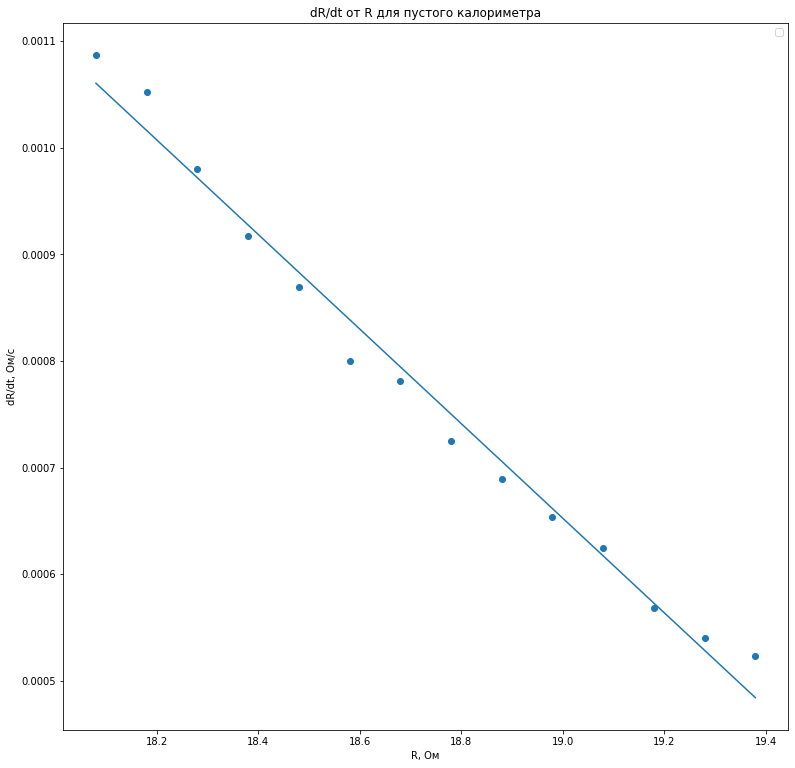
\includegraphics[scale=0.5]{g1.png}
		\end{center}
		
		\item Измеренные таким образом значения $(dR/dt)_{R=R_к}$ и $R_к$ подставим в формулу (8) и вычислим теплоемкость пустого калориметра $C_0$.
		
		$(dR/dt)_{R=R_k} = 14.24 \cdot 10^{-4}$ Ом/с, $R_k = 18.08$ Ом, $P = 10.8$ Вт \\
		$C_k = \dfrac{P \cdot R_k \cdot \alpha}{\left( \frac{dR}{dt} \right)_{T_k} \left( 1 + \alpha \cdot \Delta T_k \right)} = 538.5 \pm 17.8$ Дж/К
		
		\item Откроем калориметр и поместим в него исследуемое тело(алюминий, латунь). Подождем, пока температура калориметра с телом стабилизируется. Так как точность измерений возрастает при совпадении диапазонов изменения температуры калориметра с телом и без тела,после стабилизации температуры извлечем тело из калориметра и охладим его под струей водопроводной воды. Затем тело вытрем сухой тряпкой и дополнительно просушим его под струей сжатого воздуха из воздухопроводной сети. После этого рабочее тело вновь вставим в калориметр и, дождавшись стабилизации температуры, приступим к измерениям. Нагревание образца произведем в течение 15~---~20 минут. По полученным результатам определим величину теплоемкости образца вместе с калориметром $C_1$ . Теплоемкость исследуемого тела $C_Т$ определяется как разность теплоемкостей: $C_Т = C_1 - C_0$.
		
		\begin{itemize}
			\item Алюминий: \\
				
				\begin{tabular}{|c|c|c|c|c|c|c|c|c|} \hline
				$R, Ом$ & 18.08 & 18.18 & 18.28 & 18.38 & 18.48 & 18.58 & \multicolumn{2}{|c|}{18.68} \\ \hline
					$t, c$ & 0.0 & 108.0 & 224.0 & 348.0 & 481.0 & 619.0 & \multicolumn{2}{|c|}{772.0} \\ \hline
					$R, ом$ & 18.78 & 18.88 & 18.98 & 19.08 & 19.18 & 19.28 & 19.38 & 19.48 \\ \hline
					$t, c$ & 935.0 & 1112.0 & 1294.0 & 1488.0 & 1701.0 & 1927.0 & 2157.0 & 2389.0 \\ \hline
				\end{tabular} \\	
				
				\begin{center}
					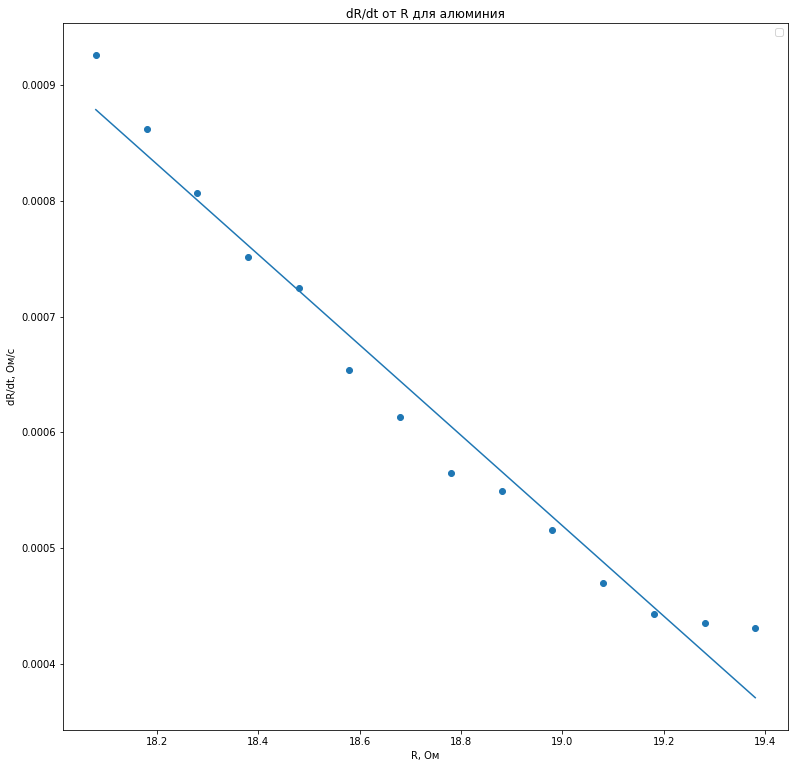
\includegraphics[scale=0.5]{g2.png}
				\end{center}								
				
				$(dR/dt)_{R=R_k} = 9.58 \cdot 10^{-4}$ Ом/с, $R_k = 18.08$ Ом, $P = 10.8$ Вт \\
		$C_{al} = \dfrac{P \cdot R_k \cdot \alpha}{\left( \frac{dR}{dt} \right)_{T_k} \left( 1 + \alpha \cdot \Delta T_k \right)} = 261.6 \pm 30.4$ Дж/К \\
		
				Тогда, удельная и молярная теплоемкости алюминия (масса алюминия: $m = 294$ г, молярная масса алюминия: $27$ г/моль): \\
				
				$C_{уд}^{al} = 889.8 \pm 103.6$ Дж/кг$\cdot$К \\ \\
				$C_{\nu}^{al} = 24.0 \pm 2.8$ Дж/моль$\cdot$К \\	
				
			\item Латунь: \\
			
				\begin{tabular}{|c|c|c|c|c|c|c|c|c|} \hline
				$R, Ом$ & 18.08 & 18.18 & 18.28 & 18.38 & 18.48 & 18.58 & \multicolumn{2}{|c|}{18.68} \\ \hline
					$t, c$ & 0.0 & 135.0 & 274.0 & 421.0 & 576.0 & 741.0 & \multicolumn{2}{|c|}{913.0} \\ \hline
					$R, ом$ & 18.78 & 18.88 & 18.98 & 19.08 & 19.18 & 19.28 & 19.38 & 19.48 \\ \hline
					$t, c$ & 1094.0 & 1285.0 & 1483.0 & 1693.0 & 1909.0 & 2135.0 & 2371.0 & 2619.0 \\ \hline
				\end{tabular} \\	
				
				\begin{center}
					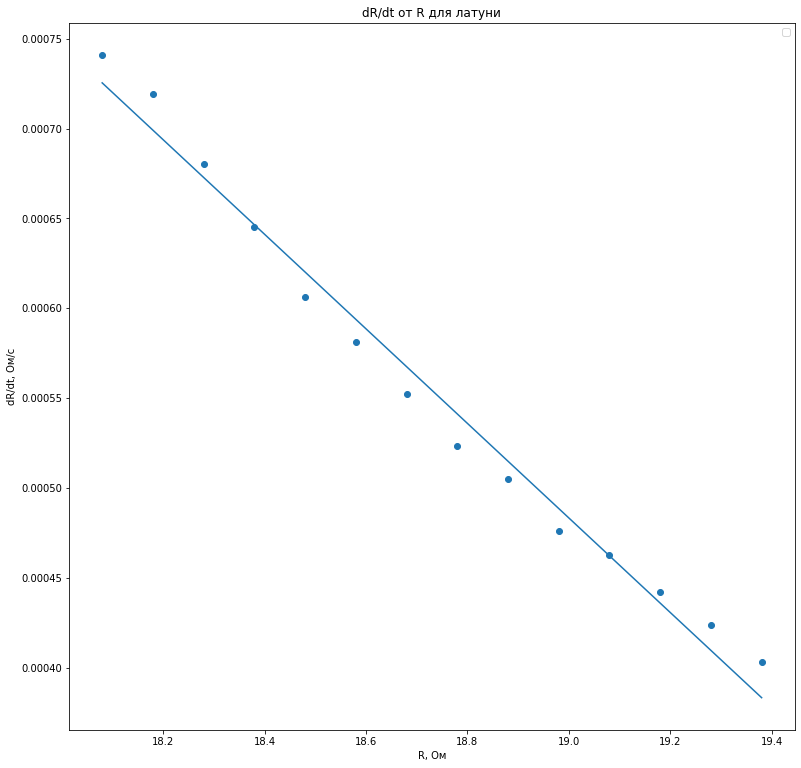
\includegraphics[scale=0.5]{g3.png}
				\end{center}
				
				$(dR/dt)_{R=R_k} = 8.89 \cdot 10^{-4}$ Ом/с, $R_k = 18.08$ Ом, $P = 10.8$ Вт \\
		$C_{la} = \dfrac{P \cdot R_k \cdot \alpha}{\left( \frac{dR}{dt} \right)_{T_k} \left( 1 + \alpha \cdot \Delta T_k \right)} = 323.3 \pm 28.6$ Дж/К \\
		
				Тогда, удельная и молярная теплоемкости латуни (масса латуни: $m = 875.5$ г, молярная масса латуни: $64.3$ г/моль): \\
				
				$C_{уд}^{la} = 369.3 \pm 32.7$ Дж/кг$\cdot$К \\ \\
				$C_{\nu}^{la} = 23.7 \pm 2.1$ Дж/моль$\cdot$К \\
		\end{itemize}
		
		\item Также на отдельном графике отобразим измеренные нами зависимости: \\
		
		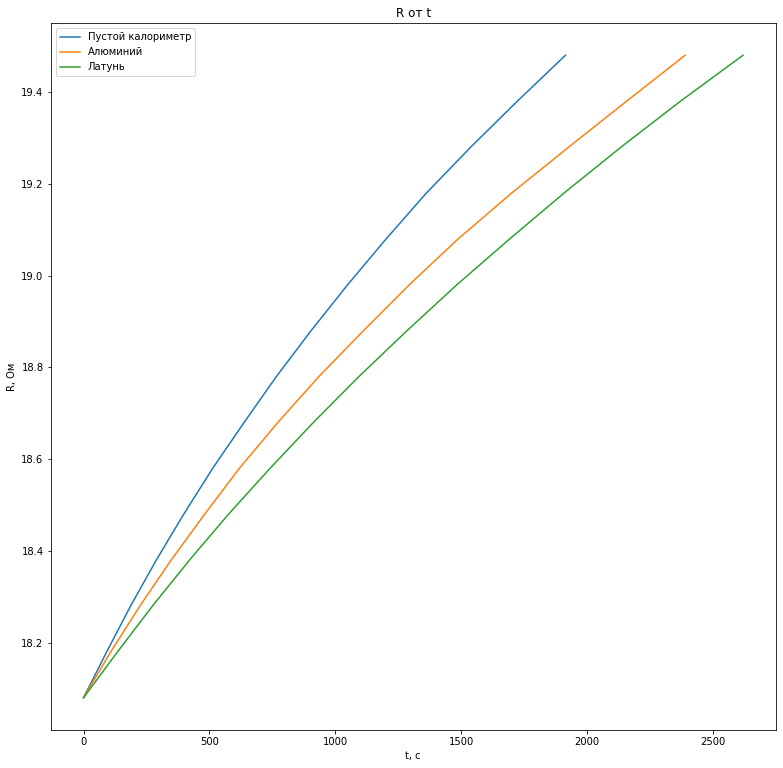
\includegraphics[scale=0.5]{g4.png}		
		
	\end{enumerate}
	
	\paragraph {Вывод:} 
		В ходе работы мною были измерены удельные теплоемкости алюминия ($C = 889.8$ Дж/кг$\cdot$K) и латуни ($C = 369.3$ Дж/кг$\cdot$K). Табличные значения составляют $C_{al} = 920$ Дж/кг$\cdot$K и $C_{la} = 380$ Дж/кг$\cdot$K. Таким образом, для алюминия ошибка составила $\mu_{al} = 3.3 \%$, для латуни~---~$\mu_{la} = 2.8 \%$
\end{document}